\chapter{METHODOLOGY}
\section{System Development Approach}
An incremental approach, also known as an iterative or step-by-step approach, is a development or problem-solving method that breaks down a larger task or project into smaller, manageable increments or steps. Rather than attempting to tackle the entire task at once, an incremental approach focuses on making incremental progress by completing and delivering smaller portions of work in a series of iterations.
\begin{itemize}
    \setlength\itemsep{0.25em}
    \item Initial Planning and Requirements Gathering
    \item Increment Planning and Design
    \item Development and Implementation
    \item Testing and Quality Assurance
    \item Evaluation and Feedback
    \item Iterative Development and Refinement
    \item Deployment and Release
    \item Repeat the Process for Subsequent Increments
\end{itemize}
\section{Requirement Analysis}
\section{Feasibility Analysis}
A feasibility study is a systematic and structured analysis conducted to determine the viability and practicality of a proposed project plan. It serves as an evaluation tool to assess whether the project can be successfully implemented and if it aligns with the organization's goals and objectives. It involves gathering and analyzing relevant information to determine if the project is technically feasible, operationally feasible, economically feasible, and scheduling feasible.
\subsection{Economical Feasibility}
Since the proposed system has a web application, we will be using free and open-source software development tools such as HTML,CSS,JS, PHP, MySQL and Figma. We will only need some economy for server for hosting.
\subsection{Operational Feasibility}
Operational feasibility for the proposed system focuses ease of use. As the system is designed to be interactive, users do not require in-depth knowledge of the mobile app to navigate and utilize its features. The user interface (UI) is specifically designed to be user-friendly, ensuring a smooth and intuitive experience. This approach minimizes the need for extensive training and reduces potential resistance from users.  
\subsection{Technical Feasibility}
There are several development technologies available. For frontend development, we have HTML,CSS,JS and React JS. For backend development, we have PHP along with the MySQL database. In our application, we have utilized HTML,CSS,JS, for the frontend and PHP with MySQL for the backend. Both HTML,CSS,JS, and PHP are open-source technologies and are supported by large companies with vibrant communities. This ensures that technical support and resources are readily available. Considering the chosen technologies and their strong community backing, the project is technically feasible.
\newpage
\section{System Design}
\subsection{Architecture Design}
The following diagram shows diagram of our Architecture. Mainly shows what are the functions can be accessed after starting our application.
\begin{figure}[H]
    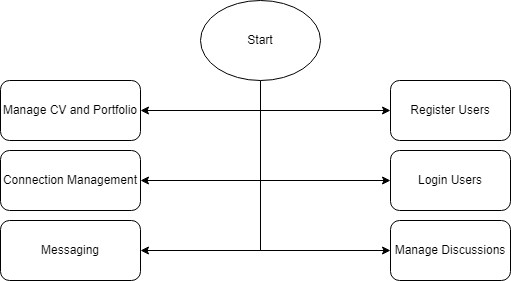
\includegraphics[height = 8cm]{Diagrams/Main_Block.png}
    \caption{Main Architecture of System}
\end{figure}
\newpage
\subsection{Data Modelling(ER-Diagram)}
ER Diagram is mainly used to design database schema. With the help of below er diagram we can easily design database in SQL.
\begin{figure}[H]
    \rotatebox{90}{
    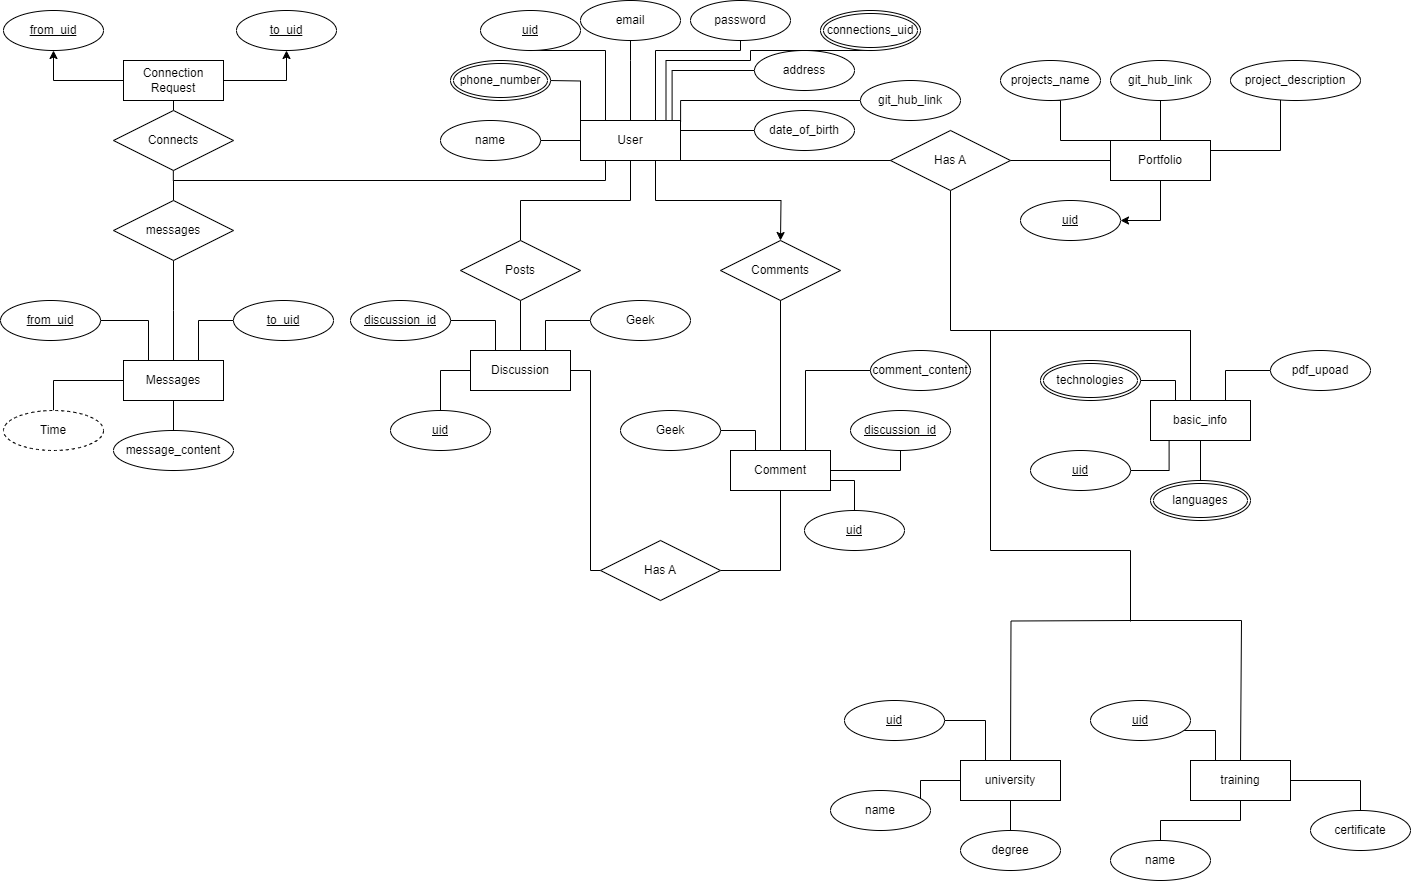
\includegraphics[height = 12cm]{Diagrams/er.drawio.png}}
    \caption{ER Diagram of System Data}
\end{figure}
\newpage
\subsection{Activity Diagram}
An activity diagram visually presents a series of actions or flow of control in a system similar to a flowchart or a data flow diagram. This diagram showed how our program flow goes on.
\begin{figure}[H]
   \centering
    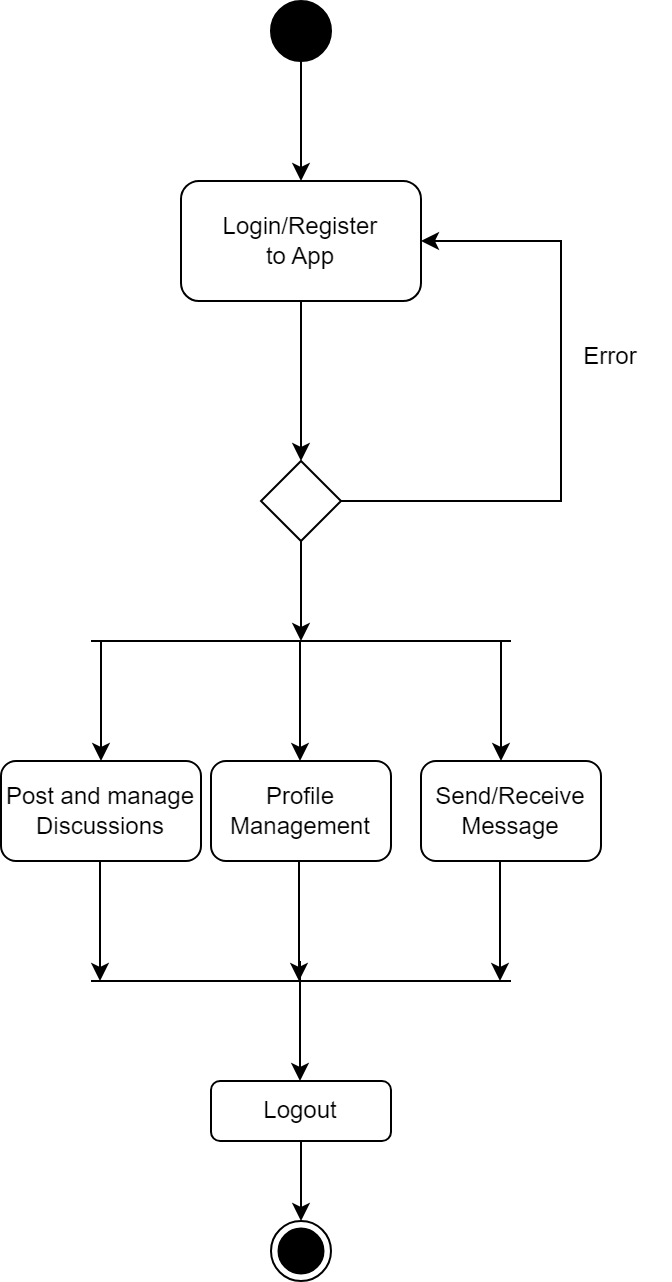
\includegraphics[height = 15cm]{Diagrams/Activity.drawio.png}
    \caption{Activity Diagram}
\end{figure}
\newpage
\subsection{DFD}
DFD or Data Flow Diagram is mainly used to show how data are being flowed in and out of our system. There are 3 levels of DFD i.e Context Level(Level 0),Level 1 and Level 2
\begin{figure}[H]
    \centering
    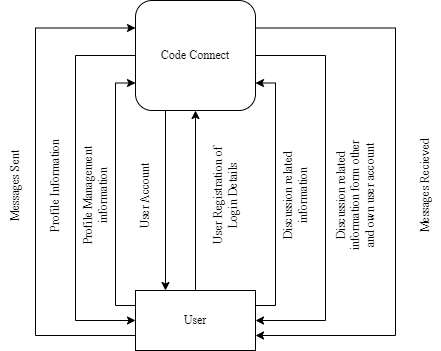
\includegraphics[height = 8cm]{Diagrams/DFD.drawio.png}
    \caption{Data Flow Diagram (Context Level)}
\end{figure}
\newpage
\subsection{Use Case Diagram}
A use case diagram, part of UML, visually represents interactions between actors and a system. Actors are external entities, while use cases depict specific functionalities. Relationships, such as association, generalization, include, and extend, illustrate connections between actors and use cases. The diagram helps in understanding system behavior, requirements, and scope.
\begin{figure}[H]
    \rotatebox{90}{
    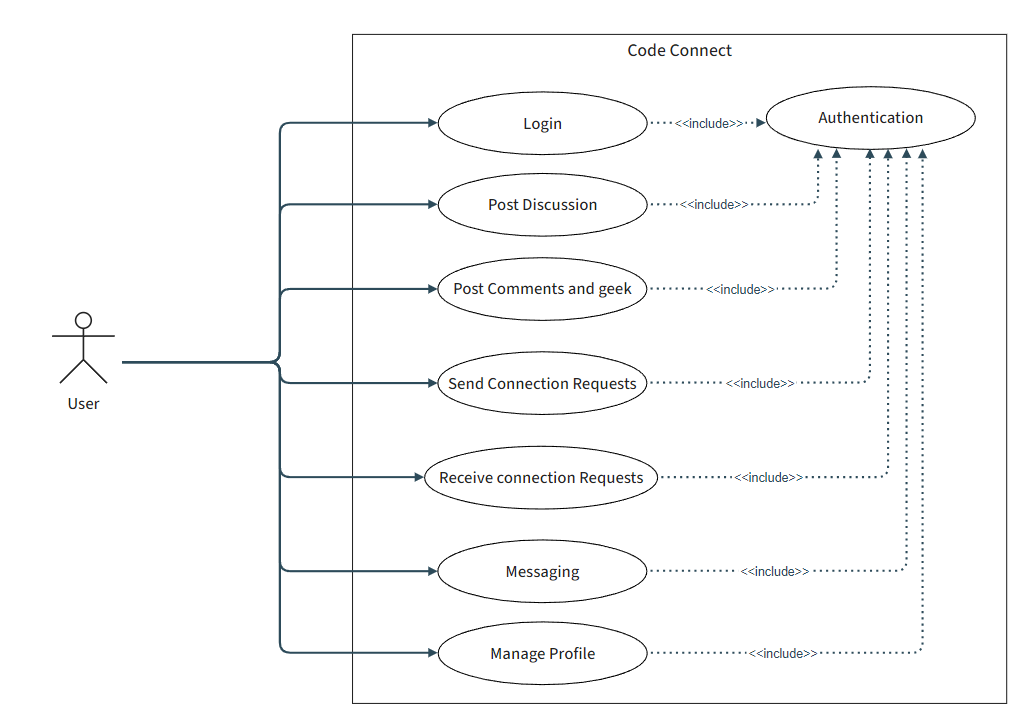
\includegraphics[height = 12cm]{Diagrams/use_case.png}}
    \caption{Use Case Diagram}
\end{figure}
